\documentclass[conference]{IEEEtran}
\IEEEoverridecommandlockouts
% The preceding line is only needed to identify funding in the first footnote. If that is unneeded, please comment it out.
\usepackage{cite}
\usepackage{amsmath,amssymb,amsfonts}
\usepackage{algorithmic}
\usepackage{graphicx}
\usepackage{textcomp}
\usepackage{xcolor}
\usepackage{wrapfig}
\usepackage{amsmath}
\usepackage{mathtools}
\usepackage[utf8]{inputenc}
\usepackage{polyglossia}
\usepackage{fontspec}
\usepackage{pbox}
\newfontface{\bn}{kalpurush.ttf}

\def\BibTeX{{\rm B\kern-.05em{\sc i\kern-.025em b}\kern-.08em
    T\kern-.1667em\lower.7ex\hbox{E}\kern-.125emX}}
\begin{document}

\title{Bangla E-Commerce Sentiment Analysis
Using Machine Learning Approach
\\


}

\author{\IEEEauthorblockN{Sunjare Zulfiker}
\IEEEauthorblockA{\textit{Department of ECE} \\
\textit{North South University}\\
Dhaka, Bangladesh \\
sunjare.zulfiker@northsouth.edu}
\and
\IEEEauthorblockN{Ankur Chowdhury }
\IEEEauthorblockA{\textit{Department of ECE} \\
\textit{North South University}\\
Dhaka, Bangladesh \\
ankur.chowdhury@northsouth.edu}
\and 
\IEEEauthorblockN{Dip Roy}
\IEEEauthorblockA{\textit{Department of ECE} \\
\textit{North South University}\\
Dhaka, Bangladesh \\
dip.roy@northsouth.edu}
\and

\IEEEauthorblockN{Shukdev Datta}
\IEEEauthorblockA{\textit{Department of ECE} \\
\textit{North South University}\\
Dhaka, Bangladesh \\
shukdev.datta@northsouth.edu}

}

\maketitle

\begin{abstract}
Nowadays, netizens often express their feelings and sentiments regarding different products on social media websites. So, many companies have become much concerned about the sentiments of the netizens towards their products and services. Furthermore, by analyzing the customers' opinions, many organizations can determine the level of client satisfaction with a particular product. Currently, plenty of E-commerce organizations have emerged in Bangladesh due to the advancement of the information and technology sector. The Bangladeshi netizens also frequently express their views and opinions on various social media websites regarding the services of these E-commerce organizations. In this study, we have constructed a Bengali corpus of the public views about the products and services of multiple Bangladeshi E-commerce organizations. Besides, we have proposed different machine learning classifiers (i.e. Multinomial Naive Bayes, Logistic Regression, Support Vector Machine, Decision Tree, Random Forest, and Stochastic Gradient Descent) to predict and analyze the polarity of public sentiments. Term Frequency–Inverse Document Frequency (TF-IDF) technique has been applied by using Trigram features. Finally, by optimizing the hyperparameters using the RandomizedSearchCV algorithm, Suppor Vector Machine (SVM) classifier showed the highest accuracy of 90.68\% for predicting the polarity of the public sentiments.
\end{abstract}

\begin{IEEEkeywords}
E-commerce, Sentiment analysis, Machine Learning, TF-IDF, Trigram, GridSearchCV 
\end{IEEEkeywords}


\section{Introduction}
The number of E-Commerce users is increasing significantly because of the comfortability, which breaks all the physical barriers. Therefore, there is a high demand for customers' opinions or product reviews by the customers that helps to judge the service and the product quality of an E-Commerce site. Over 88\% of online customers trust reviews as much as personal recommendations, according to research conducted on Amazon last year \cite{b1}. The amount of social networking site users is vast at present due to the easy access to the internet in Bangladesh. Daraz, Chaldal, Bikroy.com, and Pickaboo are some notable E-Commerce sites in Bangladesh. People express their viewpoints through text on social networking sites like Facebook, Twitter, Instagram, etc., after buying products from these E-Commerce sites. And these sentiments or viewpoints are generating massive data over social networking sites. The work of text analysis and processing is developing continuously. So, sentiment analysis in E-Commerce reviews can play a crucial role in upholding product quality and customer satisfaction.    \par
Sentiment analysis using machine learning received enormous attention in recent years. Sentiment analysis is used to assess or analyze data in text format. Hence, it helps to determine whether a text is positive or negative. With the help of sentiment analysis, it has become very easy to evaluate the polarity of a large amount of data and to help service providers and product manufacturers to fulfill their goals. \par
In this research, our main goal is to find the sentiment of products based on Bangla reviews and comments. We have collected Bangla reviews from different social sites. We have used different machine learning algorithms and used RandomizedSearchCV for hyperparameter optimization to reach accuracy at a satisfactory level. We have also extracted features from the processed data by using TF-IDF technique. \par
The major contributions of this study are as followings:
\begin{itemize}
\vspace{1mm}
\item We have constructed a Bengali corpus based on the customer reviews about the products and services of different E-commerce sites.     
\vspace{1mm}
\item Analyzed the sentiments of the Bangladeshi customers' reviews regarding the services of these E-commerce sites.
\vspace{1mm}
\item Explored different state-of-the-art machine learning algorithms and identified the best algorithm to predict the polarity of the customers' sentiments. 
\end{itemize}
The rest of the paper is organized as follows: Section II discusses about the related works of this study. Section III portrays the applied methodology for analyzing the public sentiments, the results of this study have been represented in Section IV. A comparative analysis of the results of this study and other existing works has been delineated in Section V. Finally, the paper is concluded in Section VI.  

\section{Related Works}
Sentiment analysis of subjects had been a favorite topic for researchers these days. But very few works are done on Bengali Text sentiment analysis. 
\par
Hossain et al. \cite{b2} have used many approaches to evaluate the performance of all of their models through confusion matrix, f1 score, recall, precision, ROC, and precision versus recall curve. In the case of the cross-validation technique used, they used 10-fold cross-validation on all the seven classifiers. The seven classifiers which have been chosen for their project are LR (Logistic Regression), MNB (multinomial Naive Bayes), RF (Random forest classifier), DT (decision tree classifier), KNN (K-Nearest Neighbor), SVM (Support Vector Machine) and SGD (stochastic gradient descent). Among all of these classifiers, they have found out that only four of them are giving acceptable accuracy. So they are chosen and they are LR (83\% accuracy for Uni-gram, 77\% accuracy for Bi-gram, 66\% accuracy for Tri-gram), MNB (88\% accuracy for Uni-gram, 78\% accuracy for Bi-gram, 69\% accuracy for Tri-gram), SVM (81\% accuracy for Uni-gram, 77\% accuracy for Bi-gram, 63\% accuracy for Tri-gram) and lastly SGD (77\% accuracy for Uni-gram, 72\% accuracy for Bi-gram, 68\% accuracy for Tri-gram). The researchers themselves collected their own data in a dataset from blogs, Facebook, and e-commerce sites. \par
Wahid et al. \cite{b3} have used LSTM layer to predict sentiment from their dataset which is ABSA. They were able to produce a test accuracy of 95\%. They compared their work with other works on the same dataset and they found out that those works used SVM and one of the works achieved an accuracy of 71\% and another one achieved an accuracy of 73.49\% on test set. But their LSTM model which was their proposed model and achieved a testing accuracy of 95\%. \par
Ferdous et al. \cite{b4} used TF-IDF technique for features selection. They have also used PCA which is Principal Component Analysis in order to lower the dimensions of the dataset. The dataset used is collected from Daraz. A variety of machine learning algorithms were applied to the model created from the dataset. They are Ridge Classifier (78.85\% prediction accuracy, highest among all), Logistic Regression (75.67\% prediction accuracy), SVM – Linear Kernel (75.19\% prediction accuracy), Extreme Gradient Boosting (70.43\% prediction accuracy), CatBoost Classifier (69.79\% prediction accuracy), Light Gradient Boosting Machine (69.63\% prediction accuracy), Gradient Boosting Classifier (69.32\% prediction accuracy), Extra Trees Classifier (69.16\% prediction accuracy), K Neighbors Classifier (67.25\% prediction accuracy) and Random Forest Classifier (66.61\% prediction accuracy).
\par   
Jahed et al.\cite{b5} used six machine learning algorithms for their sentiment analysis in the e-commerce industry. They used NLP techniques and collect data only from daraz.com.bd. They had developed a machine learning model where reviews on three different languages (Bangla, English, and Romanized Bangla) because Daraz reviews were mostly in three types. They demonstrated a comparative analysis with existing work and discussed the detailed accuracy, precision, recall, F1 scores, and ROC area. For three languages they prepared three datasets and collected a total of 7181 data. In their dataset, they labeled all the review data as Negative, Positive, Neutral, Slightly Negative, and Slightly Positive sentiment. They used supervised learning because, in addition, it is a classification model problem. One by one they apply all their machine learning algorithm. For the Bangla dataset, the Support Vector Machine(SVM) algorithm performed best by achieving 94\% accuracy and for the English and Romanized Bangla dataset, the Random Forest algorithm performed best by achieving 93\% and 94\% accuracy respectively.
\par
Shamsul et al.\cite{b6} made a sentiment analysis on Bangladesh cricket with a support vector machine(SVM). They choose the Bengali language and targeted a special sector which is Bangladesh Cricket where people express their opinions in their native Bengali languages. They had collected a dataset which is referred to as the Bengali dataset ABSA in their initial period to train and build their machine learning system because it is similar to cricket-related data. They worked on three sentiments of people(Negative, Positive, and Neutral). In their dataset, they labeled all the review data as Praise, Criticism, and Sadness. Finally, they targeted public posts or comments from the Facebook group of Bangladesh Cricket and the sports section of Prothom-Alo newspaper and collected about 1601 data for their main dataset. They used Python NLTK for tokenizing and used TF-IDF to vectorize the data as a feature. Using the SVM algorithm finally they achieved 64.596\% accuracy for their own dataset and for the ABSA dataset they achieved 73.490\% accuracy respectively. 
\par
Neethu et al.\cite{b7} used in sentiment analysis two main techniques which are symbolic techniques or the Knowledge base approach. For her analysis Knowledge base approach required a large database of predefined emotions and an efficient knowledge representation for identifying sentiments and the Machine learning approach makes use of a training set to develop a sentiment classifier that classifies sentiments. They used different machine learning techniques for classifying comments. They created a dataset by collecting comments for a certain period of time. They were using Naive Bayes, Support Vector Machine, Maximum Entropy, and Ensemble classifiers, and their performances are compared and got, all these classifiers have almost similar accuracy for the new feature vector.\par
Sudhanshu et al.\cite{b8} made an engineer and used the Chart Programming interface. This is an application from the Facebook engineer site. They ran the pre-processing working with information to be viable for the conclusion examination. In any case, in this examination, they have converted into English from more than 70 dialects. They were analyzing the symbolic letters and their meaning. They've compiled the acronyms most commonly used by Facebook users chatting privately. In this paper, they have followed the method of Naive Bayes classifier and Support Vector Machine where they got 71.4\% accuracy of Naive Bayes classifier and 90.88\% accuracy of Support Vector Machine. They were identified during research analysis for both Twitter and Facebook data.\par


\vspace{0.5cm}
\section{Methodology}
This section delineates the overall methods and techniques for performing sentiment analysis of the netizens' opinions regarding the E-commerce business sites of Bangladesh.

\subsection{Dataset Colection}
We have collected the dataset from different social media pages and groups. We worked only with Bangla comments and collected 1631 understandable Bangla reviews and comments. After collecting data, we labeled them manually as positive or negative.

\subsection{Dataset Analysis}
In the constructed dataset, there is a total of 1631 reviews. Among these reviews, 862 reviews are positive, and the rest 769 reviews are negative. So, the percentages of the positive and negative reviews in the dataset are 52.9\% and 47.1\%, respectively. Figure 1 shows the percentages of the positive and negative reviews in the constructed dataset.
\begin{figure}[htbp]
  \centering
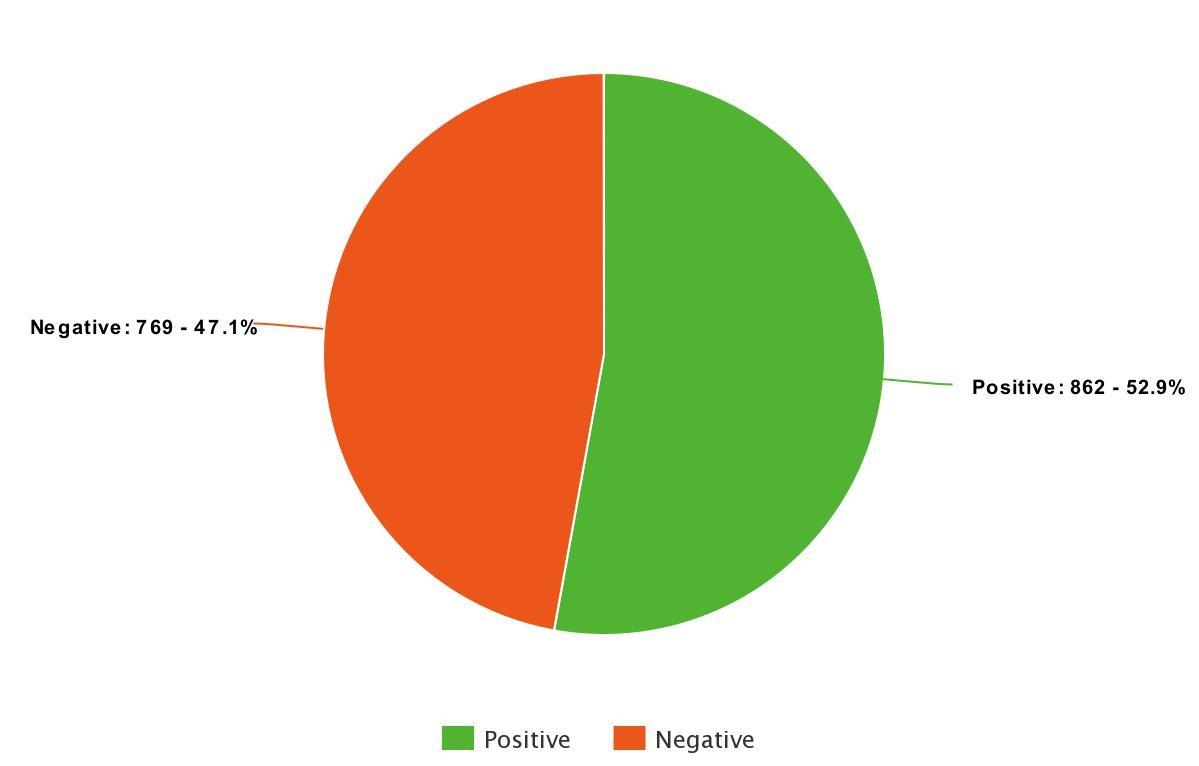
\includegraphics[width=\columnwidth,height=\textheight,keepaspectratio]{dataset.jpeg}
  \caption{Percentages of the Positive and Negative Reviews in the Dataset}
  \label{fig:scope1}
\end{figure}
\vspace{0.5cm}

We have also generated word clouds for the positive and the negative reviews. Figure 2 shows the word cloud for the reviews having positive polarities. From Figure 2, it can be found that the frequencies of the words \bn "ভালো", "আলহামদুলিল্লাহ", "ধন্যবাদ", "সুন্দর" are higher than the other words in the positive reviews, and so, the size of these words are comparatively larger than the other words in the word cloud.

\begin{figure}[htbp]
  \centering
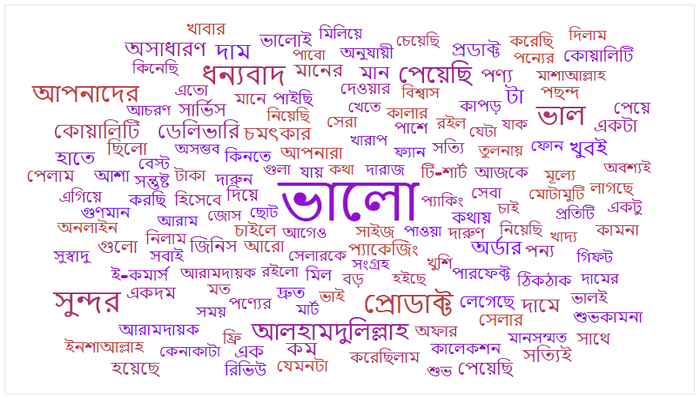
\includegraphics[width=\columnwidth,height=\textheight,keepaspectratio]{snipvaloPNG.PNG}
  \caption{Word Cloud for Positive Reviews}
  \label{fig:scope1}
\end{figure}

On the contrary, Figure 3 shows the word cloud for the negative reviews. Figure 3 portrays that the frequencies of the words \bn "বাজে", "দাম", "খারাপ", "না", "নাই", and "টাকা"  are more significant in the negative reviews than the other words. 

\begin{figure}[htbp]
  \centering
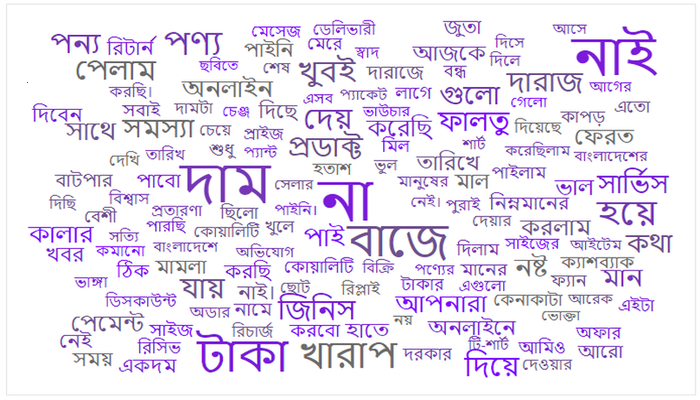
\includegraphics[width=\columnwidth,height=\textheight,keepaspectratio]{snipkharap.png}
  \caption{Word Cloud for Negative Reviews}
  \label{fig:scope1}
\end{figure}


\subsection{Implementation Steps}
Fig. 4 shows the overall implementation steps of this study for predicting the polarity of the sentiments of the customers' reviews.

\begin{figure}[htbp]
  \centering
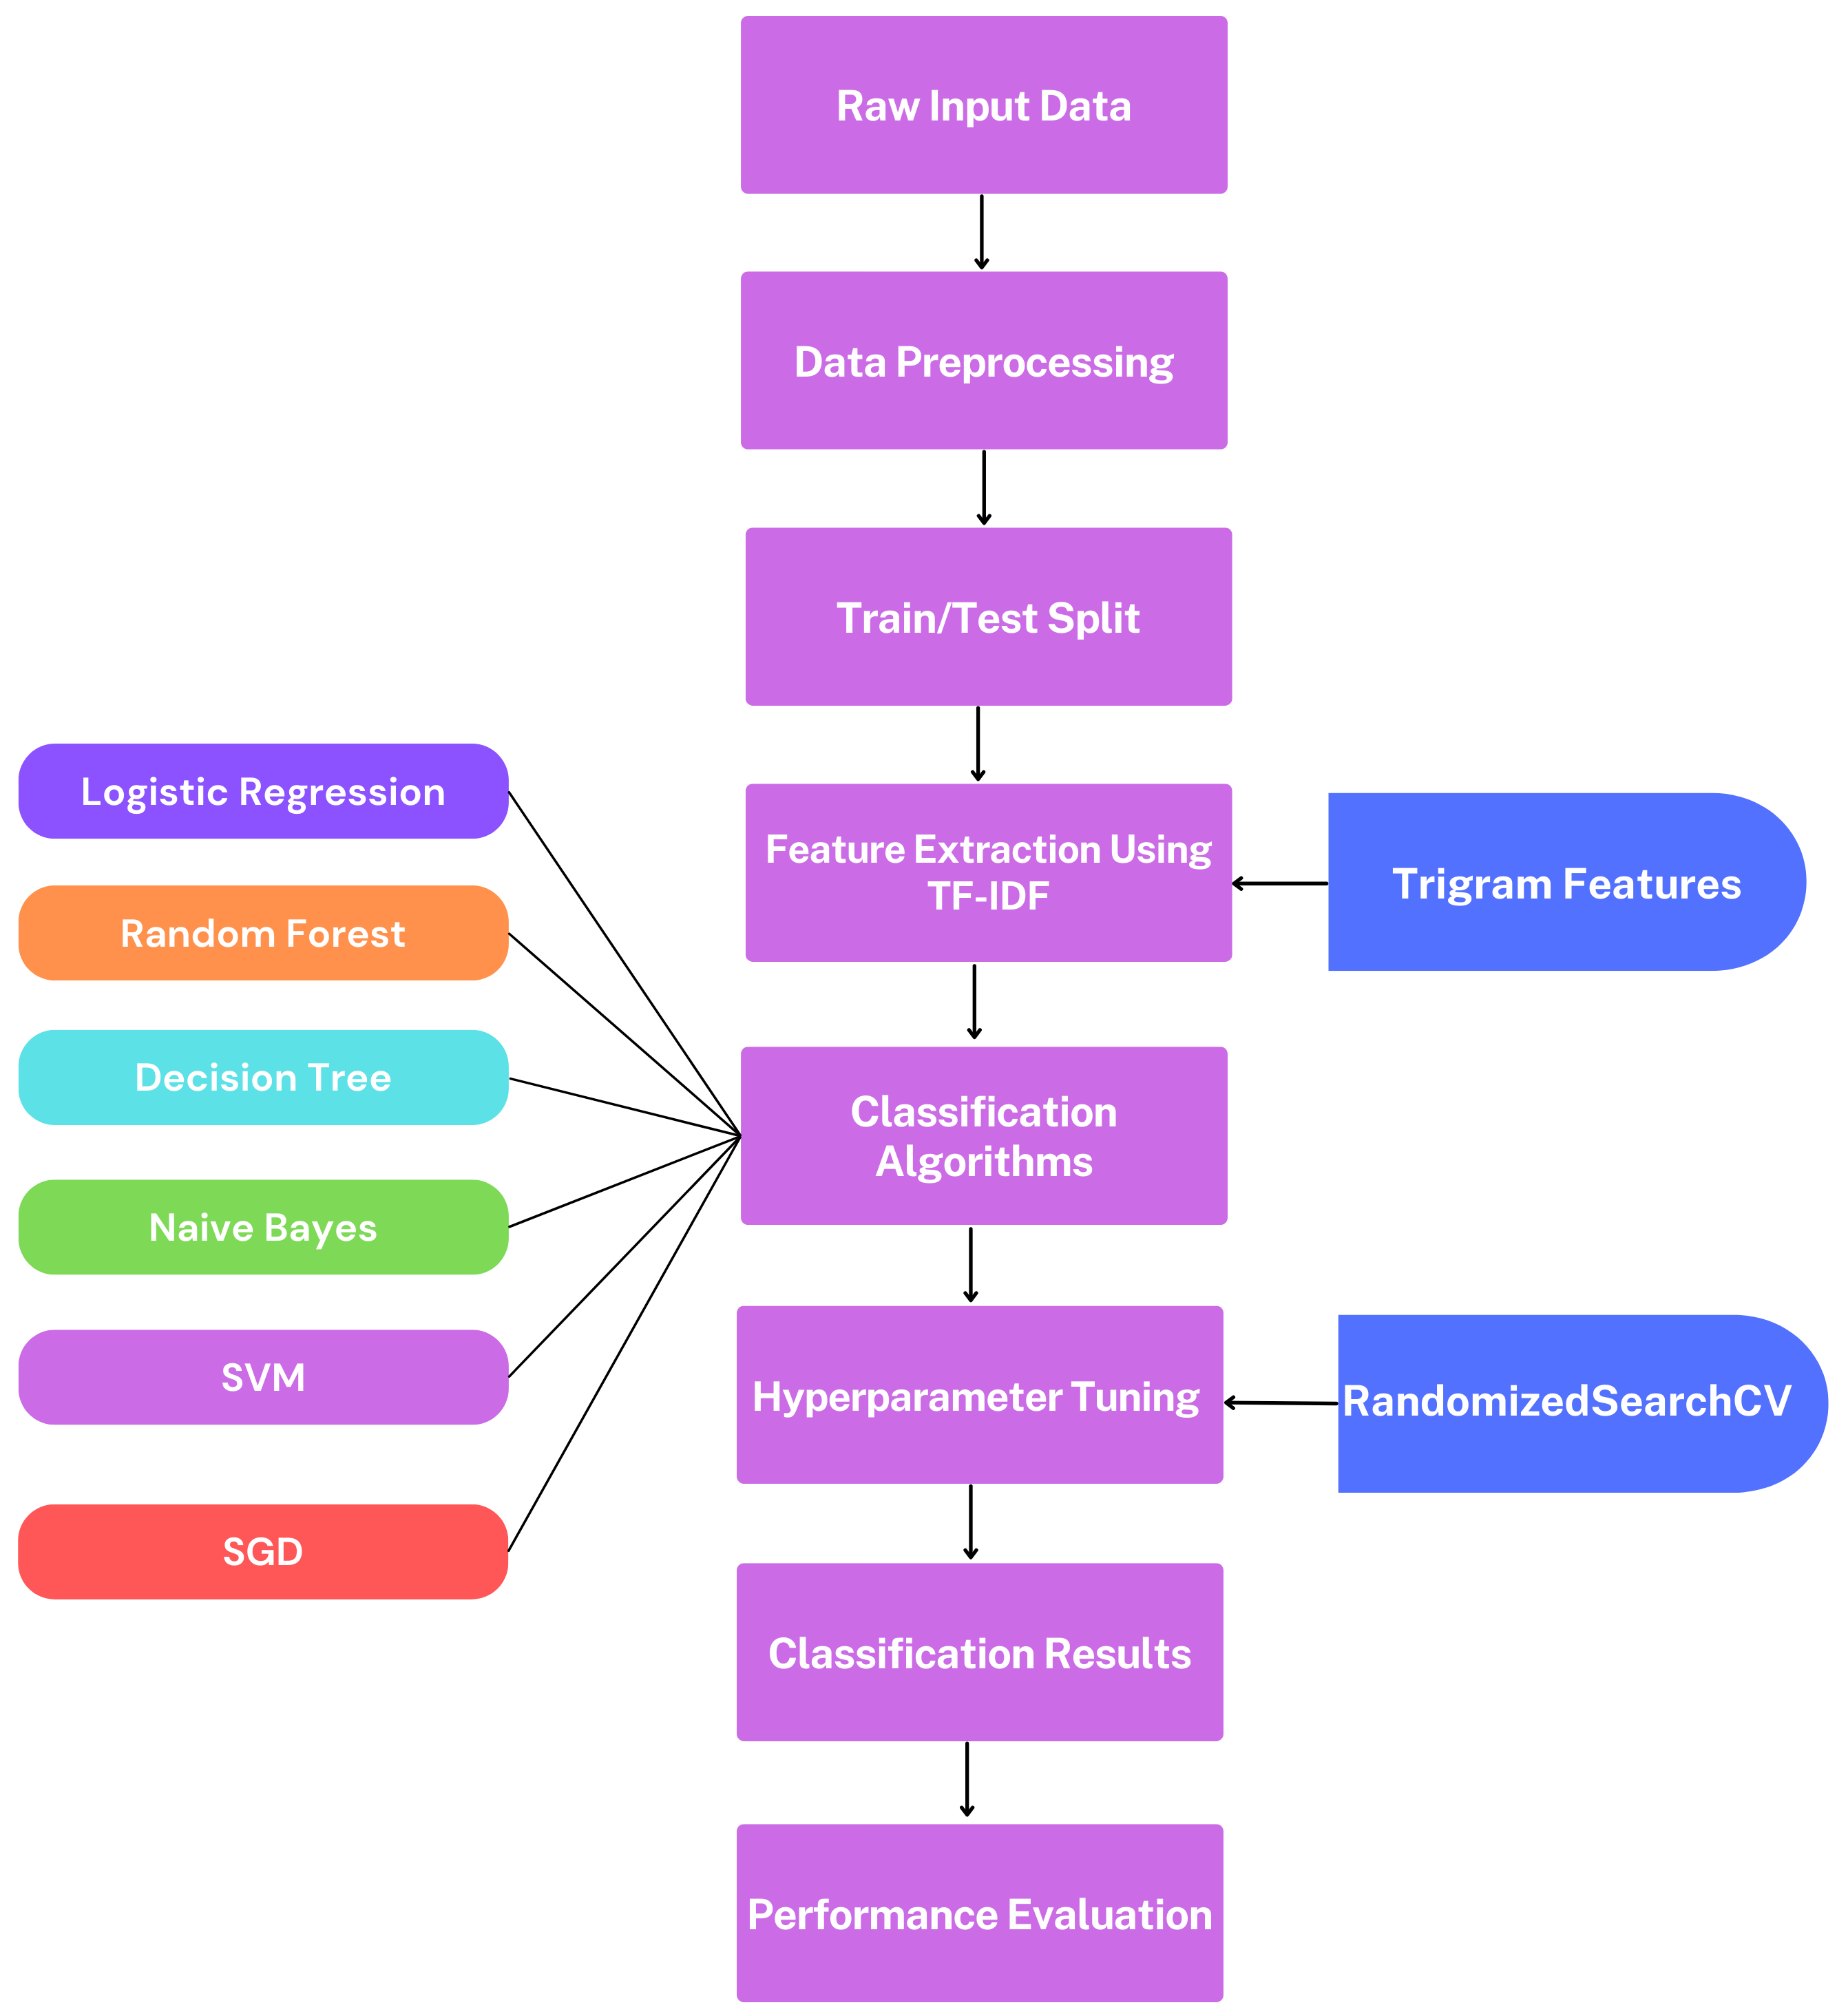
\includegraphics[width=\columnwidth,height=\textheight,keepaspectratio]{methodology.png}
  \caption{Step by Step Procedures for Predicting the Polarity of the Sentiments}
  \label{fig:scope1}
\end{figure}


\subsubsection{Data Preprocessing}
Real-world data are very messy, so we have to do data preprocessing to get higher accuracy. We preprocessed our data step by step. All the steps of preprocessing are shown below.

\begin{itemize}
\vspace{1mm}
\item 	Tokenization: It is the process of separating strings into words. Tokens can be individual words, punctuation marks, or emojis. Here, tokenization was used to tokenize each review.   
\vspace{1mm}
\item 	Removing Punctuation marks: After tokenizing each sentence, we removed all the punctuation marks from the tokenized sentence as they do not carry any value in detecting sentiment.
\vspace{1mm}
\item 	Removing Stop Words:  Stop words are those words that do not have any impact on analyzing sentiment. So, we called the stopwords library from bltk(Bengali Natural Learning Processing Toolkit) and removed those stopwords from the tokenized sentences.
\vspace{1mm}

\end{itemize}

Furthermore, we did manual preprocessing, like removing emojis, hashtags, etc.

\vspace{4mm}
\subsubsection{Train/Test Split}
In this step, we have split the preprocessed dataset into test and train data. We have used 75\% data of our dataset to train the machine learning models, and the remaining 25\% data of the dataset have been used for testing.
\vspace{4mm}

\subsubsection{TF-IDF Using Trigram Features}

The dataset should be in a numerical format to fit the data into machine learning models. Therefore, we have converted the sentence into numbers, and this technique contains two terms: TF (Term Frequency) and IDF(Inverse Document Frequency). Where TF is the frequency of a word in a document and IDF is the significance of that word in a document. In this work, we have selected trigram features where trigram is the three consecutive words in a sentence. TF and IDF can be computed by Equations (1), and (2), respectively.
\par

\begin{equation}
\begin{multlined}
   \textbf{Term Frequency, } TF=\\\frac{The\:number\:of\:appearance\:of\:a\:term\:T\:in\:the\:document }{Total\:number\:of\:terms\:in\:the\:document}
 \end{multlined}
\end{equation}

\begin{equation}
\begin{multlined}
    \textbf{Inverse Document Frequency, }IDF=\\log_e\frac{Total\:number\:of\:documents}{Number\:of\:documents\:having\:term\:T}
\end{multlined}
\end{equation}



\subsubsection{Classification Algorithms}
After doing feature extraction using TF-IDF we used 6 different classifiers to predict the sentiment. 
\par 
\vspace{0.3cm}
\textbf{Logistic regression (LR)} is never used in regression problems. It is actually used in classification problems. Usually, Logistic regression is used in binary classification problems. Unlike Linear regression, Logistic regression's range is bounded between 0 and 1, and also it does not need the linear relationship between input and the target variable. 
\\
Equation 3 shows the logistic function. 
\begin{equation}
   \textbf{Logistic Function, } h_\Theta(x)=\frac{1}{1 + e^{-x}}
\end{equation}


\par
\vspace{0.3cm}

Decision Tree (DT) is a classifier that is used in supervised Learning and can be used in regression and classification Problems. It has a tree-like structure where the root represents the dataset and the branch represents the decision rules and each leaf node represents the outcome of the action. It is the graphical representation of all the possible results of different actions. 

\par
\vspace{0.3cm}
Random forest (RF) is a special type of classifier that is used in Supervised Learning Problems. It consists of number of decision trees on various subsets of the given dataset and it takes the majority vote for classification and in the case of regression, it takes the average of all the output of the decision trees. The higher the number of decision trees in the RF classifier, the higher will be the accuracy. The majority vote will be counted.   

\par

\vspace{0.3cm}
Naive Bayes (NB) is an algorithm that is commonly used in Supervised Learning and mainly used for solving classification Problems. It is frequently used in text classification problems which include a large dataset with high dimensionality. The main thing about this classifier is that it is a probabilistic classifier which means that it predicts the target on the basis of the probability of an object. Naive Bayes works on the basis of the Bayes Theorem. The equation for the Bayes Theorem can be found in Equation 4, where P(A|B) is the posterior probability, P(B|A) is likelihood probability, P(A) is prior and P(B) is marginal probability. 

\begin{equation}
   P(A|B)=\frac{P(B|A) P(A)}{P(B)}
\end{equation}
 In this study, we have used the Multinomial Naive Bayes.

\vspace{0.3cm}

\par 
Support Vector Machine (SVM) is one of the most popular algorithms that is used in supervised learning. This algorithm can be used both in classification and regression problems but usually, it is more popular for classification problems. The objective of SVM is to create a straight line that will distinctly separate two classes if it is a binary problem, and when there is new data, the decision boundary will clearly identify in which class the new data lies. 
\par
\vspace{0.3cm}

In Stochastic Gradient Descent (SGD), a few of the samples will be selected randomly instead of using the whole dataset for each iteration. SGD is extremely useful when you are dealing with a huge dataset. The typical Gradient Descent (GD) algorithm works on the whole dataset for each iteration. %Usually working on the whole dataset for each iteration makes it easy to find the values of $\theta$  for which cost function is %minimum, but this is not good for huge datasets. 
But it is not a good practice for huge datasets. Because to complete every iteration, GD uses all the samples in the dataset until the values of $\theta$ is found for which the cost function is minimum. In such a scenario, SGD uses a single sample for each iteration and the sample is randomly shuffled and chosen to perform the iteration. \\

% For i in range (m):
% \begin{align*}
% \Theta_{j} = \Theta_{j} - \alpha(\hat{y}^{i} - y^{i}) x^{i}_{j}
% \end{align*}

\vspace{0.3cm}
\subsubsection{Hyperparameter Tuning}
After predicting the polarity of the sentiments, we selected the classifier that gave the maximum accuracy and performed hyperparameter optimization of that classifier using the RandomizedSearchCV algorithm. In our work, the SVM model was giving the best accuracy, so we performed hyperparameter optimization of the SVM classifier.

\vspace{0.3cm}
\subsubsection{Performance Evaluation}
In this step, we have compared the performance of different machine learning models by utilizing different performance metrics, like Accuracy, Precision, Recall, and F1-Score. Based on these performance metrics, we have concluded our study by determining the best model for predicting the polarity of public sentiments. 



\section{Results And Discussions}
In this section, we have evaluated the performance of our classifiers using some performance metrics. Before discussing different measures, there are a few terms we need to understand, and they are- Confusion Matrix, Accuracy, F1-Score, Precision, and Recall. 
\\
\\
\textbf{Confusion Matrix:} A table called a confusion matrix is used to describe how well a classification system performs. The output of a classification algorithm is shown and summarized in a confusion matrix. Confusion Matrix is a useful technique that allows for measuring Recall, Precision, Accuracy, and AUC-ROC curve. Figure 5 shows a Confusion Matrix. 
\begin{figure}[htbp]
  \centering
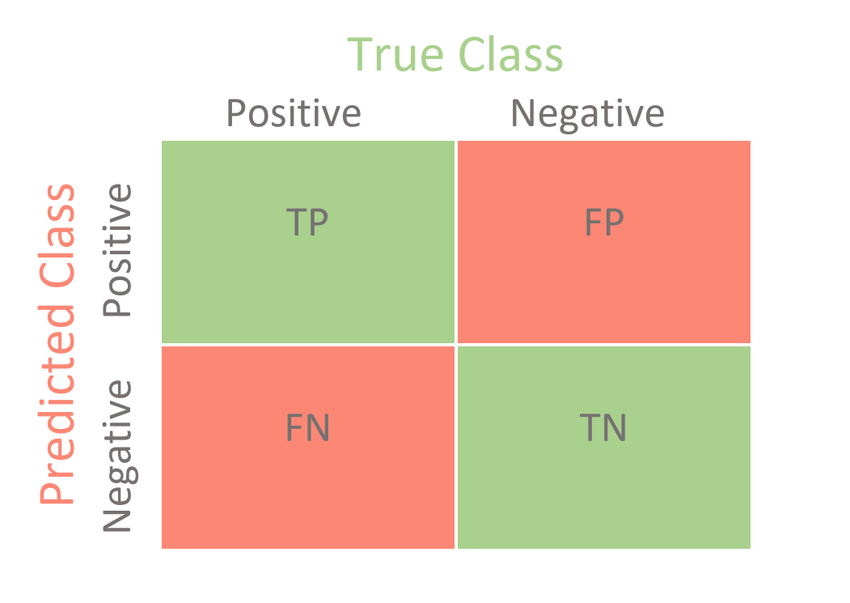
\includegraphics[width=\columnwidth,height=\textheight,keepaspectratio]{confusion.png}
\caption{Confusion Matrix}
  \label{fig:scope1}
\end{figure}
\\
The details for TP, TN, FP, and FN in Figure 5 are stated below.
\begin{itemize}
\vspace{1mm}
\item 	\textbf{True Positive (TP):} True Positive represents the number of actually positive data that were predicted as positive by a classifier.
\vspace{1mm}
\item 	\textbf{True Negative (TN):} True Negative portrays the number of actually negative data that were predicted as negative by a classifier.
\vspace{1mm}
\item 	\textbf{False Positives (FP):} It depicts the number of actually negative data that were identified as positive by a classifier. 

\vspace{1mm}
\item 	\textbf{False Negative (FN):} It denotes the number of actually positive data that were identified as negative by a classifier.

\end{itemize}
% \begin{itemize}
% \vspace{1mm}
% \item 	\textbf{True Positive (TP):} True positive represents the quantity of correctly identified data.
% \vspace{1mm}
% \item 	\textbf{False Positives (FP):} False positives are instances of correctly classified data that were misclassified.

% \vspace{1mm}
% \item 	\textbf{False Negative (FN):} False Negative refers number of incorrect data classified as correct. misclassified.
% \vspace{1mm}
% \item 	\textbf{True Negative (TN):} True Negative refers the numbers of incorrect data classified.

% \end{itemize}



\textbf{Accuracy:} Accuracy predicts how frequently the classifier makes the correct prediction. It is the ratio between the number of correct predictions and the total number of predictions. Accuracy can be measured by Equation 5.

\begin{equation}
   Accuracy=\frac{TP+TN}{TP+TN+FP+FN}
\end{equation}



\vspace{0.5cm}
\textbf{Precision:} A classification model's capacity to isolate and identify only the relevant data items. How many of the return documents are accurate is a measure of precision for a classifier. Lower accuracy results in more false positives, while better precision results in fewer false positives. Precision can be measured by Equation 6.

\begin{equation}
  Precision = \frac{TP}{TP+FP}
\end{equation}

\vspace{0.5cm}
\textbf{Recall:} The recall is determined by dividing the total number of Positive samples by the proportion of Positive samples that were correctly identified as Positive. Less false negatives are a result of the higher recall. Recall assesses a model's capacity to identify Positive samples. More positive samples are found when the recall is higher. Recall can be measured by Equation 7.
\begin{equation}
  Recall = \frac{TP}{TP+FN}
\end{equation}

\vspace{0.5cm}
\textbf{F1-Score:} The F1-Score combines the precision and recall of a classifier into a single metric by calculating their harmonic mean. It is a weighted average of precision and recall. As we know in precision and in recall there is a false positive and false negative, so F1-Score also consider both of them. It is mainly used to compare the performance of two classifiers. F1-Score can be measured by Equation 8.
\begin{equation}
  F1-Score = \frac{2*TP}{2*TP+FP+FN}
\end{equation}
\\
Here, Table I shows the confusion matrix of the different classifiers that we have used in this study.

\begin{table}[h]
\caption{Confusion Matrix for Different Classifiers}
\setlength{\tabcolsep}{8pt} % Default value: 6pt
\renewcommand{\arraystretch}{1.5} % Default value: 1
\begin{tabular}{|l|l|l|l|l|}
\hline

\textit{\textbf{Classifiers}} & \textit{\textbf{TN}} & \textit{\textbf{FP}} & \textit{\textbf{FN}} & \textit{\textbf{TP}} \\ \hline
NB & 167 & 37 & 13 & 191 \\ \hline
LR & 165 & 39 & 13 & 191 \\ \hline
DT       & 187 & 17  & 47 & 157 \\ \hline
SVM                 & 179 & 25  & 14 & 190 \\ \hline
RF       & 149 & 55  & 13 & 191 \\ \hline
SGD                 & 177 & 27  & 16 & 188 \\ \hline
SVM with RandomizedSearchCV                 & 180 & 24  & 14 & 190 \\ \hline

\end{tabular}

\end{table}



% \hspace{0.1cm}

Table II shows the performance metrics of the different classifiers for predicting the polarity of the customers' sentiments. We have calculated the Accuracy, Precision, F1-Score, and Recall of the models.


\begin{table}[h]
\caption{Performance Metrics of Different Classifiers}
\setlength{\tabcolsep}{5pt} % for width
\renewcommand{\arraystretch}{2.5} % for length
\begin{tabular}{|l|l|l|l|l|}
\hline
{\textbf{Classifiers}} & \textbf{Accuracy} & \textbf{Precision} & \textbf{Recall} & \textbf{F1-Score} \\ \hline
NB & 87.75\% & 83.77\% & 93.63\% & 88.43\% \\ \hline
LR & 87.25\% & 83.04\% & 93.63\% & 88.02\% \\ \hline
DT       & 84.31\% & 90.23\% & 76.96\% & 83.07\% \\ \hline
\textbf{{SVM}} & \textbf{{90.44\%}}  & \textbf{{88.37\% }} & \textbf{{93.14\%}} & \textbf{{ 90.69\%}} \\ \hline
RF    & 83.33\% & 77.64\% & 93.63\% & 84.89\% \\ \hline
SGD                 & 89.46\% & 87.44\% & 92.16\% & 89.74\% \\ \hline
\textbf{{\pbox{20cm}{SVM with \\ RandomizedSearchCV}}}                 & \textbf{{90.68\%}} & \textbf{{88.79\%}} & \textbf{{93.14\%}} & \textbf{{90.91\%}} \\ \hline
\end{tabular}
\end{table}

    First, of all, we applied Naive Bayes and got an accuracy of 87.75\%. and obtained precision of 83.77\%, recall 93.63\%, and F1-score of 88.43\%.  However, we got the lowest accuracy from the Random Forest classifier (83.33\%), Decision Tree slightly performs well than Random forest and we got an accuracy of 84.31\%. We got decent accuracy from Logistic regression and got an accuracy of 87.25\%. Moreover, from SGD classifier we got the second maximum accuracy of 89.46\%. SVM classifier gives us the maximum accuracy of 90.44\% among all the classifiers without optimization, the precision of 88.37\%, recall of 93.14\%, and F1-score 90.69\%. Then we applied RandomizedSearchCV for hyperparameter tuning the SVM classifier and got the highest accuracy of 91.68\% where precision is 88.79\%, recall 93.14\%, and F1-score 90.91\%. From Table II it is clear that the SVM classifier with RandomizedSearchCV outperforms all the classifiers. Furthermore, the precision, recall, and F1-score are all at their highest. 
    \\
   \hspace{1cm}
   
 Here, we can see the ROC curve for different classifiers

\begin{figure}[thpb]
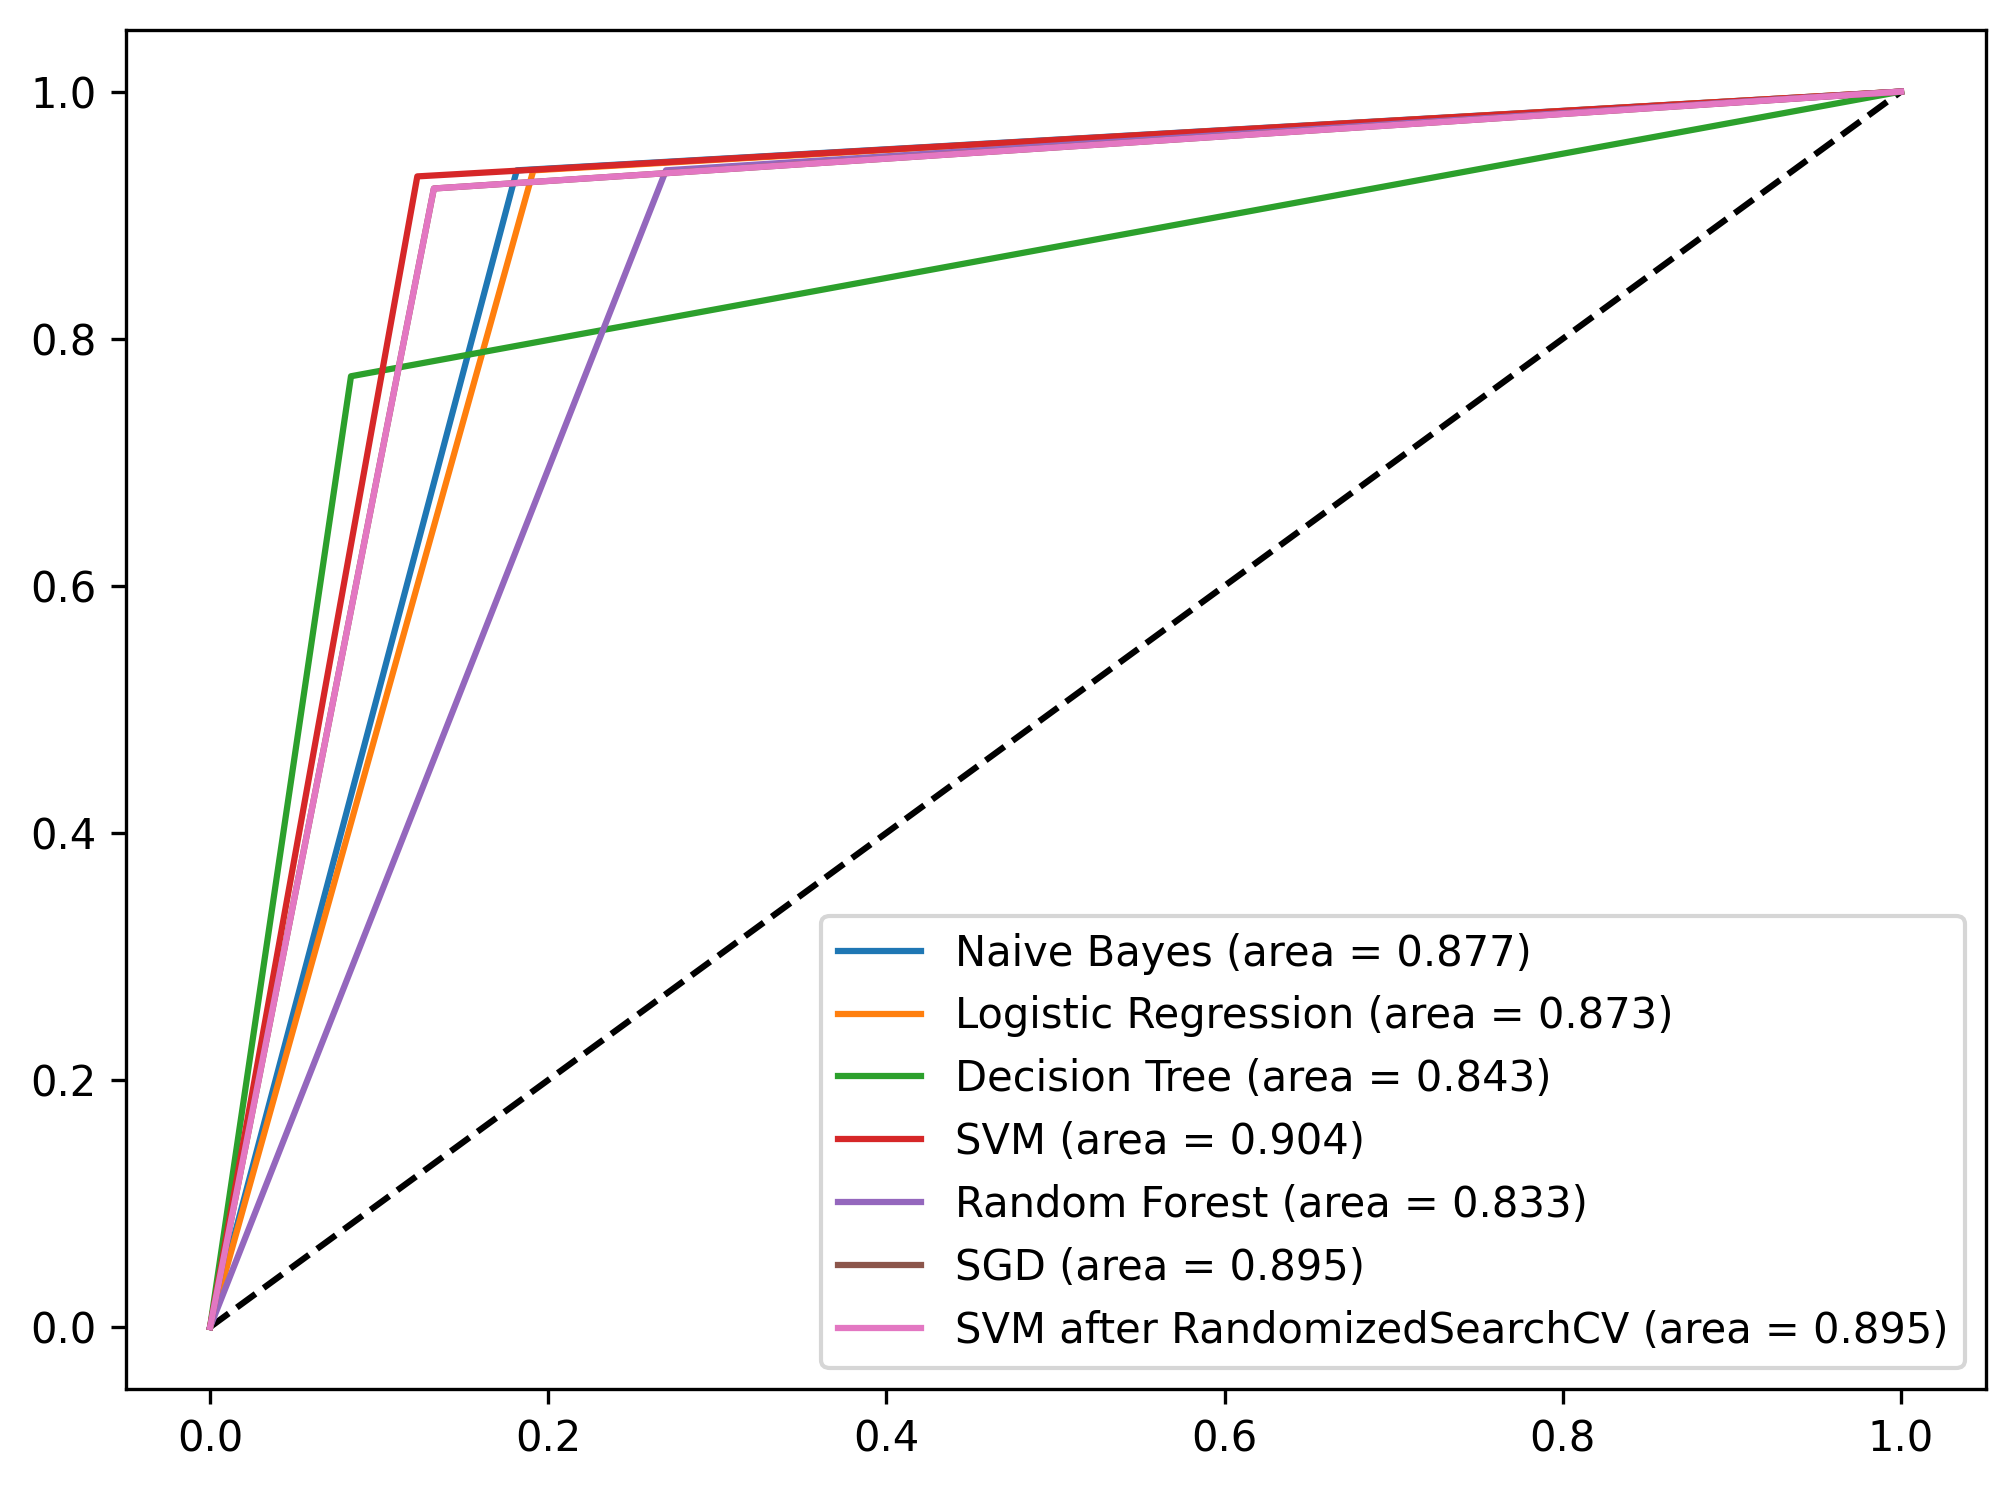
\includegraphics[width=0.5\textwidth]{ROC.png}
\caption{ROC Curve of the classifiers}
\end{figure}

In Figure 6 the x-direction of this ROC curve represents the False Positive Rate and the y-direction represents the True Positive Rate. We know that when a ROC curve is closer to the top-left corner of the graph then that specific classifier is giving better performance. Therefore, in this study SVM Classifier is in the most top-left corner of this graph. Therefore, the AUC of SVM classifier without hyperparameter tuning is maximum which is 0.904 
\vspace{0.5cm}
\section{Comparative Analysis With Existing Works.}

In this section, we have compared our study with other related works. We have evaluated these studies based on their accuracy. A comparative study between this work and other existing works are represented in Table III.
\begin{table}[h]
 \caption{Comparative Study between this Work and Other Existing Works}

\renewcommand{\arraystretch}{3} % Default value: 1

    \begin{tabular}{|p{3.5cm}|p{0.8cm}|p{1.5cm}|p{1.5cm}|}
   
    \hline
        \textbf{Research} & \textbf{Year} & \textbf{Dataset} & \textbf{Accuracy} \\ \hline
        

                
        Amazing: A sentiment mining \& Retrieval System\cite{b9} & 2009 & Customer reviews (English)  & 87.60\% \\ \hline
        
        Sentiment analysis of customer product reviews using machine learning\cite{b10} & 2017 & Amazon customer reviews (English)  & 81.75\% \\ \hline
        
        Aspect-Level Sentiment Analysis on E-Commerce Data \cite{b11} & 2018 & Amazon customer reviews (English) & 90.4\% \\ \hline

        Sentiment Analysis in E-commerce Using SVM on Roman Urdu Text\cite{b12} & 2019 & DarazPK customer reviews (Roman Urdu) & 60.90\% \\ \hline
        
        Product Review Sentiment Analysis by Using NLP and Machine Learning in Bangla Language \cite{b13} & 2020 & E-Commerce product reviews (Bangla) & 88.81\% \\ \hline
        


        Proposed model & 2022 & Product reviews (Bangla) & 90.68\% \\ \hline
    \end{tabular}
\end{table}

The above table shows the related works of different researchers. They applied different methods. Their methods of data preprocessing and feature extraction are different. Even the language of the dataset are different.  We tried to optimize some data preprocessing and feature extraction in our proposed model. Therefore, we got higher accuracy than all of these related works. 





\vspace{0.5cm}


\section{CONCLUSION}
This paper presents an approach for analyzing the sentiment of E-commerce comments in Bangla Text. In this work, various machine learning algorithms have been used to classify the implicit sentiment of customer reviews. By utilizing different traditional classifiers, we got decent accuracy. Among these classifiers, the optimized SVM classifier has provided the maximum accuracy of 90.68\%.
\\
We believe that our system can decrease customers' anxiety while shopping online. They will know the positive and negative reviews of other customers. It can be also helpful for the sellers because they can later improve the quality of their product.  In future, we will improve the performance of our model by using advanced machine learning and deep learning approaches and also include more data for our dataset.

%\section{REFERENCES}

\begin{thebibliography}{00}

\bibitem{b1}
T. U. Haque, N. N. Saber, and F. M. Shah, “Sentiment analysis on large scale amazon product reviews,” in 2018 IEEE International Conference on Innovative Research and Development (ICIRD), 2018, pp. 1–6. 39
\\
\bibitem{b2}
E. Hossain, O. Sharif, and M. Moshiul Hoque, “Sentiment polarity detection on
bengali book reviews using multinomial naive bayes,” in Progress in Advanced
Computing and Intelligent Engineering. Springer, 2021, pp. 281–292.
39
\\
\bibitem{b3}
M. F. Wahid, M. J. Hasan, and M. S. Alom, “Cricket sentiment analysis from
bangla text using recurrent neural network with long short term memory model,”
in 2019 International Conference on Bangla Speech and Language Processing
(ICBSLP), 2019, pp. 1–4.
\\

\bibitem{b4}
M. J. Ferdous, P. Sarker, and N. A. Turzo, “Assortment of bangladeshi e-commerce
site reviews using machine learning approaches,” in 2020 2nd International Con-
ference on Sustainable Technologies for Industry 4.0 (STI). IEEE, 2020, pp.
1–6.
40

\\
\bibitem{b5}
M. J. Hossain, D. D. Joy, S. Das, and R. Mustafa, “Sentiment analysis on reviews
of e-commerce sites using machine learning algorithms,” in 2022 International
Conference on Innovations in Science, Engineering and Technology (ICISET),
2022, pp. 522–52
\\
\bibitem{b6}
S. Arafin Mahtab, N. Islam, and M. Mahfuzur Rahaman, “Sentiment analysis on
bangladesh cricket with support vector machine,” in 2018 International Confer-
ence on Bangla Speech and Language Processing (ICBSLP), 2018, pp. 1–4.
40
\bibitem{b7}
M. S. Neethu and R. Rajasree, “Sentiment analysis in twitter using machine learn-
ing techniques,” in 2013 Fourth International Conference on Computing, Commu-
nications and Networking Technologies (ICCCNT), 2013, pp. 1–5.
40
\\

\bibitem{b8}
S. Tiwari and A. Sinha, “Sentiment analysis of facebook data using machine learn-
ing,” International Journal of Innovative Research in Applied Sciences and Engi-
neering, vol. 4, pp. 2456–8910, 2020.
40
\\

\bibitem{b9}
Q. Miao, Q. Li, and R. Dai, “Amazing: A sentiment mining and retrieval system,”
Expert Systems with Applications, vol. 36, no. 3, pp. 7192–7198, 2009.
41
\\

\bibitem{b10}
Z. Singla, S. Randhawa, and S. Jain, “Sentiment analysis of customer product
reviews using machine learning,” in 2017 International Conference on Intelligent
Computing and Control (I2C2), 2017, pp. 1–5.
\\
\bibitem{b11}
S. Vanaja and M. Belwal, “Aspect-level sentiment analysis on e-commerce data,”
in 2018 International Conference on Inventive Research in Computing Applica-
tions (ICIRCA), 2018, pp. 1275–1279.
41
\\
\bibitem{b12}
 F. Noor, M. Bakhtyar, and J. Baber, “Sentiment analysis in e-commerce using
svm on roman urdu text,” in Emerging Technologies in Computing, M. H. Miraz,
P. S. Excell, A. Ware, S. Soomro, and M. Ali, Eds. Cham: Springer International
Publishing, 2019, pp. 213–222

\\

\bibitem{b13}
 M. A. Shafin, M. M. Hasan, M. R. Alam, M. A. Mithu, A. U. Nur, and M. O.
Faruk, “Product review sentiment analysis by using nlp and machine learning
in bangla language,” in 2020 23rd International Conference on Computer and
Information Technology (ICCIT), 2020, pp. 1–5.
41




\end{thebibliography}


\vspace{12pt}



\end{document}
